% ---
% Arquivo com a Introdução do Trabalho de Conclusão de Curso dos alunos
% Gabriel Takaoka Nishimura, Felippe Demarqui Ramos e Vivian Kimie Isuyama
% da Escola Politécnica da Universidade de São Paulo
% ---
	\chapter*[Introdução]{Introdução} %(exemplo de capítulo sem numeração, mas presente no Sumário)
	\addcontentsline{toc}{chapter}{Introdução}
	
	\section*{Objetivos}\label{sec-objetivos}
	
	Há um aumento em escala global no uso de comunicação sem fio\cite{load-balancing}. Apenas no ano de 2015, mais de meio bilhão de telefones celulares foram adicionados à rede de telefonia no mundo \cite{cisco-forecast}. Em relação ao crescimento de aparelhos conectados como carro, geladeiras, TV’s, DVD’s, entre outros, existem previsões de que a sua quantidade chegará a 9 bilhões em 2020, com um crescimento de 900\% em relação a 2015 \cite{erricson-report}. O tráfego IP também fica cada vez mais denso, com previsão de que atinja 168 exabytes em 2019, como pode-se observar na \autoref{figure:intro-cisco}.

	\begin{chart}[ht!]
		\caption{\label{figure:intro-cisco}Crescimento do tráfego IP do ano 2014 ao 2019}
		\begin{center}
			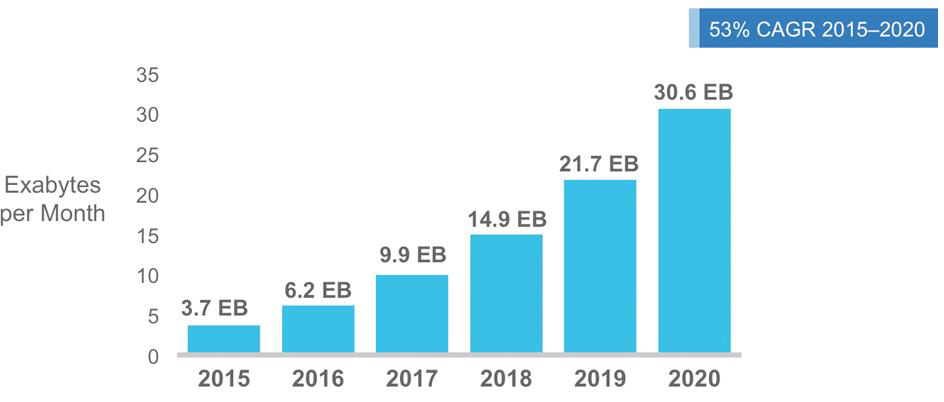
\includegraphics[scale=0.5]{cisco_exabytes_per_month.png}
		\end{center}
		\legend{Fonte: Cisco Visual Networking Index: Global Mobile Data Traffic Forecast Update, p. 5}
	\end{chart}
	
	 Esse tipo de comunicação engloba diferentes tecnologias de transmissão e recepção de dados, incluindo algumas ainda pouco exploradas. Nesse sentido, surge um interesse relevante por uma tecnologia explorada há um período relativamente curto de tempo: a transferência de dados utilizando o espectro da luz visível (Haas, 2011). Essa comunicação é conhecida como VLC (Visible Light Communication) e posteriormente, com o uso de LED's, criou-se uma nova categoria, chamada de Li-Fi (Light Fidelity) \cite{what-is-lifi}. \par

	A partir do conhecimento dessas tecnologias, discutem-se alternativas para desenvolvê-las e utilizá-las de fato. Desta maneira, apresenta-se o cerne deste estudo, que é encontrar uma forma de realizar comunicação por luz visível e implementá-la. Dentre os estudos e referências que servem a esse propósito, a norma IEEE 802.15.7 \cite{lifi-standard}(Li-Fi) se destaca como uma fonte confiável para o desenvolvimento de tecnologias nesta área. Portanto, complementa-se o problema inicial, e o principal objetivo do projeto torna-se estabelecer comunicação por luz visível através da norma IEEE 802.15.7. \par
	
	Em suma, o grupo tem o intuito de criar um transmissor em formato de luminária e um receptor anexado a um terminal, que pode ser um computador ou um dispositivo móvel. A comunicação deve ser simplex entre os dois módulos criados, para que o transmissor envie dados ao receptor, de modo a se trabalhar entre duas camadas físicas, a princípio. Posteriormente, podem-se integrar os módulos desenvolvidos a camadas mais altas, como Enlace, Rede, Transporte ou Aplicação. \par
	
	Finalmente, o escopo principal pode ser dividido em três partes:	
	\begin{itemize}
		\item |	Implementar em hardware uma das camadas definidas na norma IEEE 802.15.7;
		\item |	Estabelecer transmissão e recepção de sinais entre um LED e um fotodiodo;
		\item |	Integrar hardware digital e analógico.
	\end{itemize}

	\section*{Motivação}\label{sec-motivacao}
		
	No Brasil, a Anatel regulamenta uma banda de frequências que pertencem ao intervalo  de 3KHz até 300GHz \cite{faixa-anatel}. Isso significa que existem frequências reservadas para tipos específicos de comunicação, com o intuito de diminuir possíveis interferências entre elas. No entanto, essa atribuição deixa aparelhos como telefones sem fio, tablets, roteadores e notebooks em frequências de livre uso, como 2.4GHz. Eventualmente, o número excessivo de dispositivos conectados em  frequências livres pode causar interferência em áreas mais densas. Uma alternativa para reduzir essa possível saturação seria buscar comunicação pela luz visível, cuja frequência pertence ao intervalo de 430THz a 750THz \cite{vision}, e que não é regulamentada por nenhuma agência (vide \autoref{figure:intro-fcc}). \par
	
	\begin{figure}[h!]
		\caption{\label{figure:intro-fcc}Caracterização dos espectros de frequências, de 0Hz a 1000THz - frequências reguladas estão em laranja.}
		\centering
		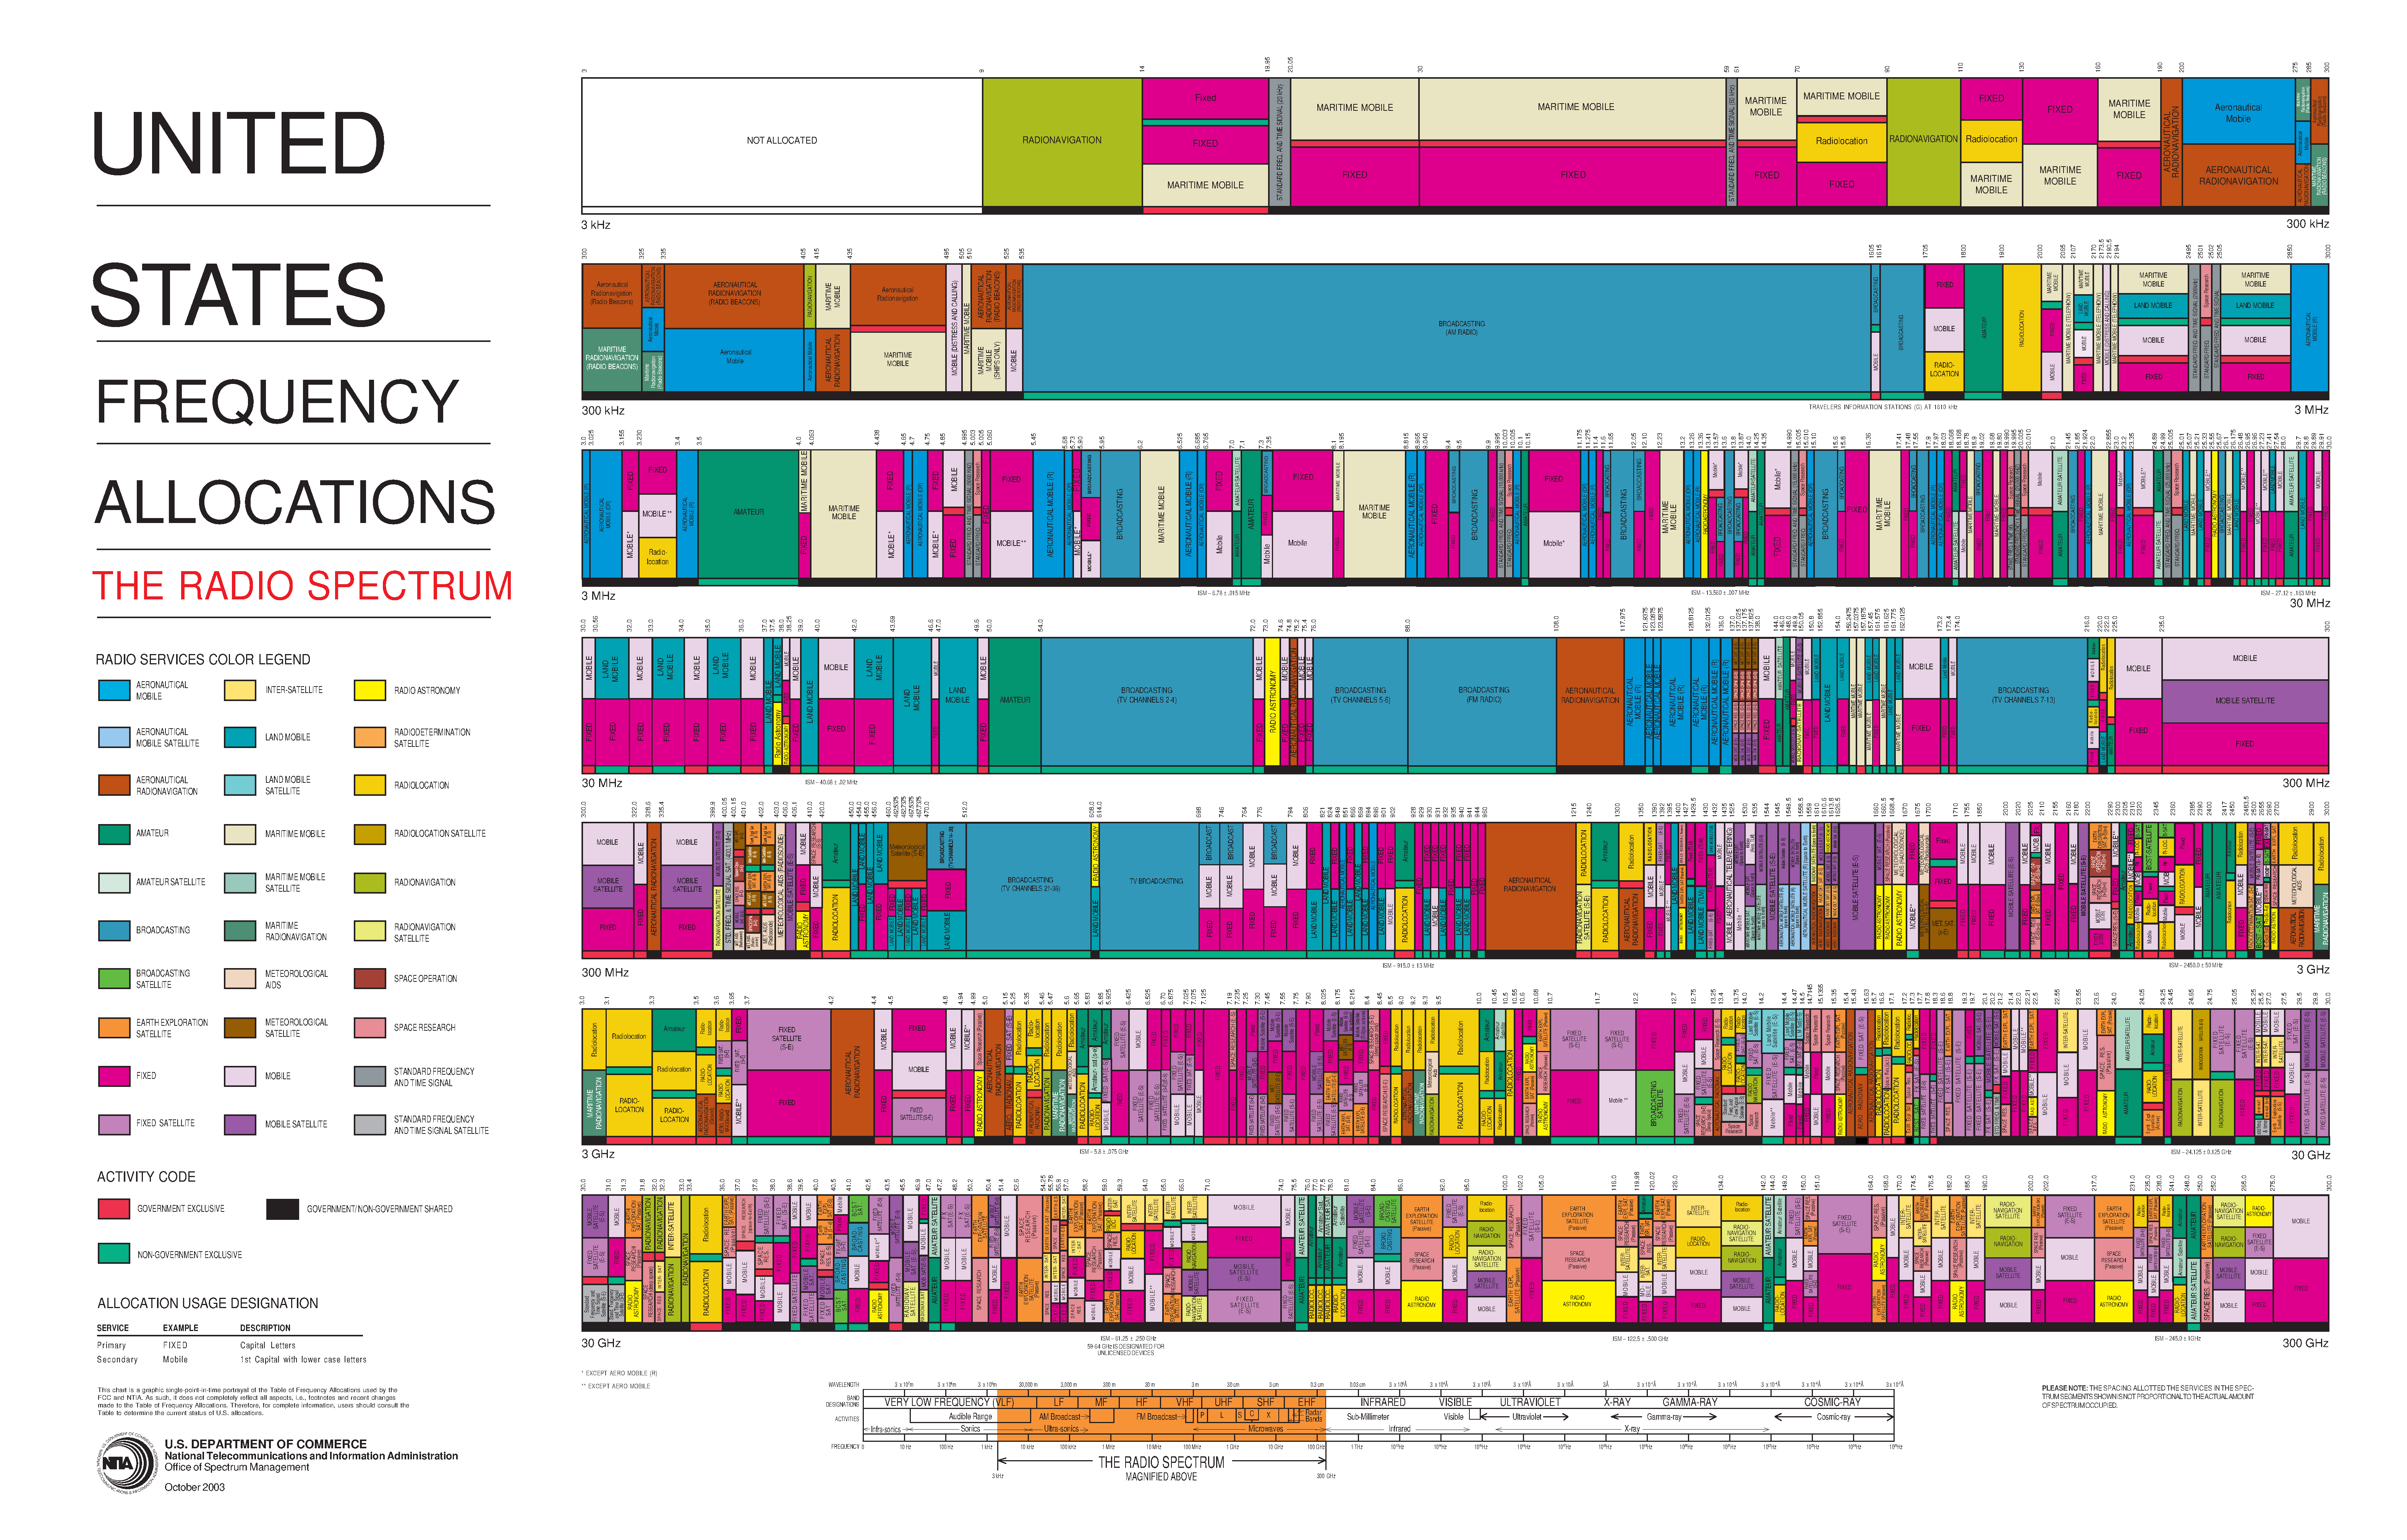
\includegraphics[width=\textwidth, trim={36.5cm 3.1cm 40cm 61cm},clip]{2003-allochrt.pdf}
		\legend{Fonte: U.S. Frequency Allocation Chart}
	\end{figure}
	
	Ademais, o uso da tecnologia Li-Fi oferece algumas vantagens \cite{comparison-wifi}. Não há, por exemplo, interferência com as bandas convencionais (como 2.4GHz e 5GHz), sendo portanto compatível com infraestruturas híbridas. Com a largura de banda 10000 vezes maior do que a de RFC, é possível hospedar uma quantidade muito maior de clientes. Nota-se também uma eficiência energética do Li-Fi, pois o LED utilizado na transmissão pode aproveitar a infra-estrutura de iluminação já existente em ambientes internos, o que justifica e reforça o uso de LED. Em sequência, pode-se citar o diferencial de que a luz não atravessa paredes, garantindo segurança e privacidade à rede. \par
	
	É importante ainda ressaltar que este projeto tem como antecedentes experiências com comunicação via luz visível. Nascidas no contexto de uma disciplina de laboratório de processadores, as principais motivações foram a maior eficiência energética da VLC, bem como a diminuição de interferência com ondas de radiofrequência. No entanto, essas experiências esbarraram em desafios, principalmente relacionados à falta de um padrão de comunicação e de componentes adequados. Além disso, houve problemas relacionados à capacidade de processamento do microcontrolador utilizado, o que é consequência de um levantamento de requisitos incompleto.

	Finalmente, este projeto surge como um amadurecimento dos objetivos anteriores. Neste segundo momento, foi escolhida uma norma que atendesse às expectativas de implementar comunicação por luz visível de forma eficiente. O padrão IEEE 802.15.7 é vantajoso por dois grandes motivos:
	(I) sua finalização em 2011, o que facilita a adequação do projeto e (II) este se encontra consolidado entre companhias e grupos industriais que formam o Consórcio Li-Fi.
